%% Tex spellcheck
% Maybe put this as Chapter 2

% Write in English.
\chapter{Chapter 2 : State of the art}

We want to use \gls{pcb} coils to move a magnet directly via the magnetic field generated by the coil. This concept is not new and has been used in some motor applications for example. There also is some people that use this concept for learning or entertainement purposes. This helped us to get some ideas on how to design our own system.

\section{PCB Motors}

There has been a huge interest in the development of \gls{pcb} motors. These motors are made by etching a coil pattern on a \gls{pcb} to act as the stator. There is a center shaft attached to magnets. When powering the coils in a specific sequence, the magnets will be attracted to the coils and the motor will rotate.

\begin{figure}[H]
	\centering
	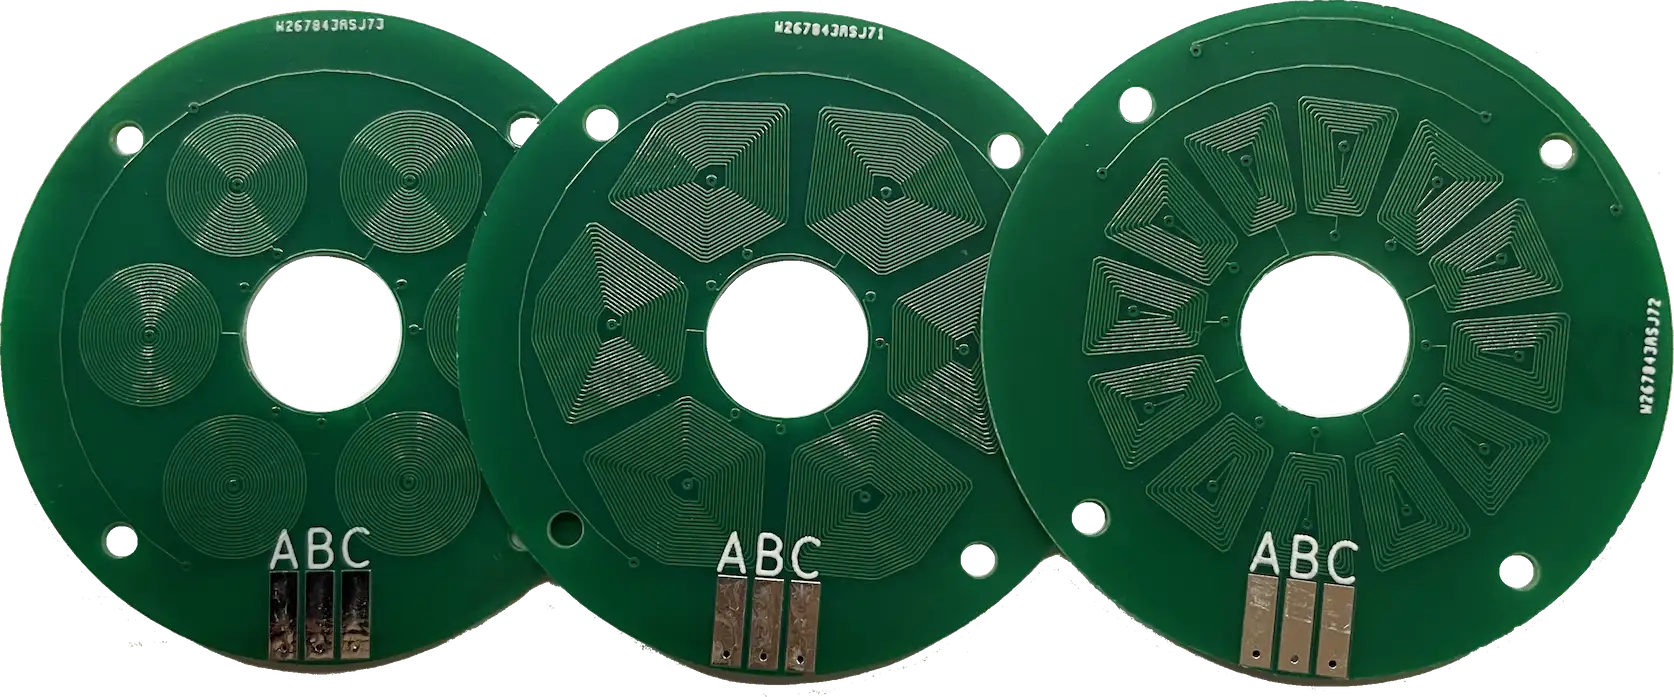
\includegraphics[width=0.8\linewidth]{pcb_motor.png}
	\caption[\gls{pcb} Motor]{Atomic14 \gls{pcb} stators Source: https://www.atomic14.com ref: URL02}
	\label{fig:pcb_motor}
\end{figure}

There also is some commercial products that use this concept. They claim to be more efficient, Lighter with higher torque density. For example \footcite{noauthor_pcb_nodate} sells services and production to design your own \gls{pcb} motor with specified specs, and they use \gls{pcb} stators.

\begin{figure}[H]
	\centering
	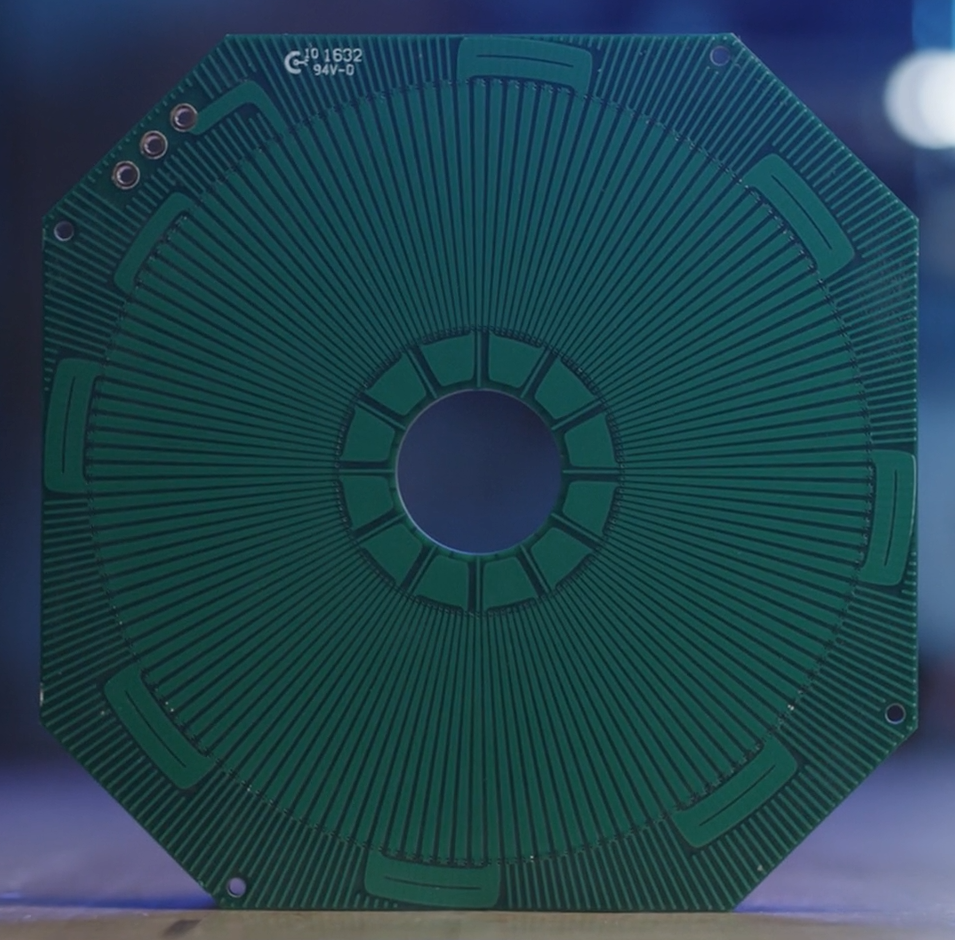
\includegraphics[width=0.8\linewidth]{pcb_stator_actual.png}
	\caption[Commercial \gls{pcb} Motor's stator by ECM]{\gls{pcb} stator from EMC Source: https://pcbstator.com/ ref: URL03}
	\label{fig:pcb_stator}
\end{figure}

\begin{figure}[H]
	\centering
	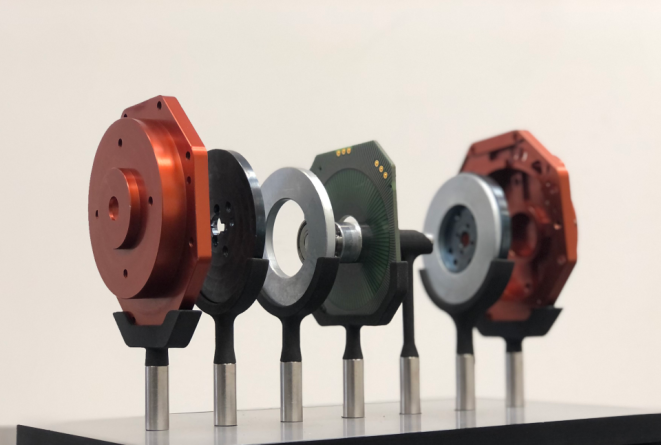
\includegraphics[width=0.8\linewidth]{commercial_pcb_motor.png}
	\caption[Commercial \gls{pcb} Motor by ECM]{\gls{pcb} Stator's full motor design Source: https://pcbstator.com/ ref: URL04}
	\label{fig:pcb_stator_full}
\end{figure}


\section{PCB 2D linear actuators}

There are some people that have used the same concept to make a linear actuator. They use linear \gls{pcb} traces to move a magnet in a 2D linear fashion. There is for example a project on hackaday \footcite{noauthor_2d_nodate} that does just that. They actually use 3 different for each axis. They alternate those 3 coils made with \gls{pcb} traces to move the magnet in the desired direction.

The concept seems to have been developped and tested by SRI\footcite{sri_magnetically_2014} in 2014. They used a similar concept to move a micro robot in a 2D space.

\begin{figure}[H]
	\centering
	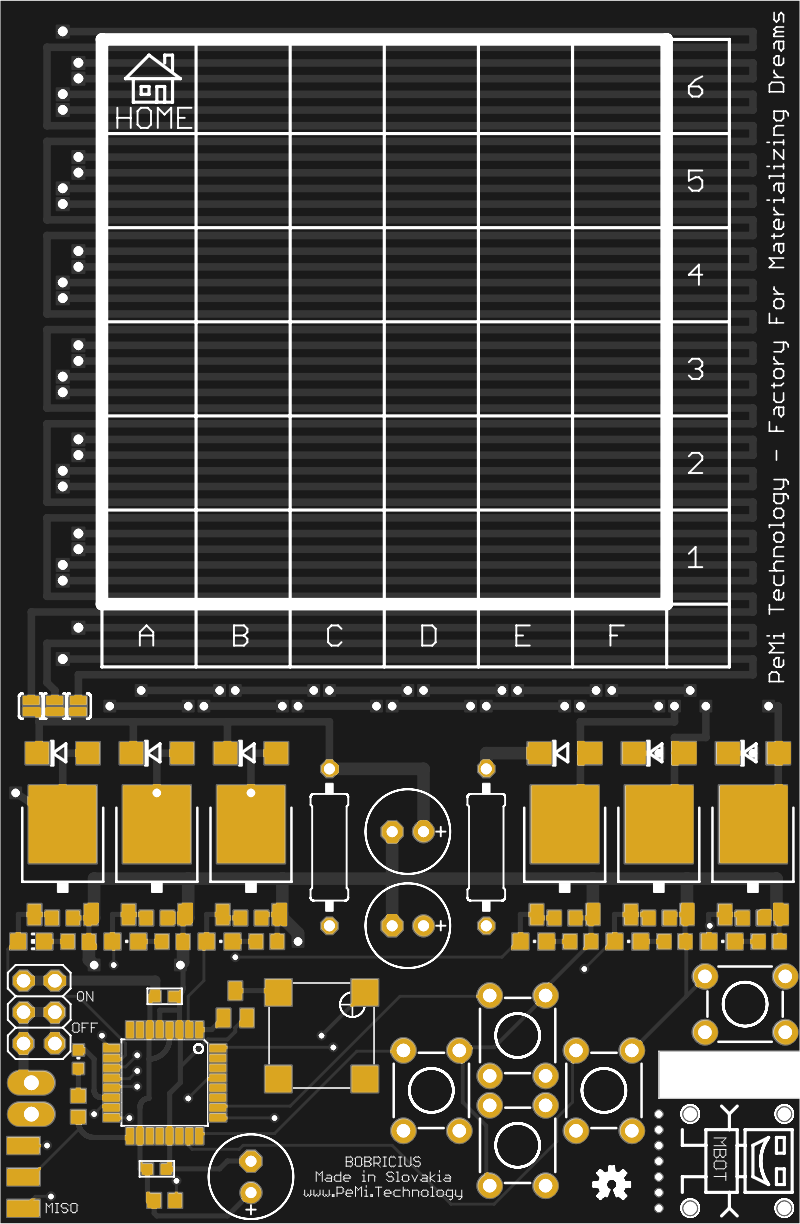
\includegraphics[width=0.5\linewidth]{2d_pcb.png}
	\caption[2D X/Y \gls{pcb} actuator by Bobricius]{\gls{pcb} move a magnet in X/Y axis  Source: hackaday.io ref: URL06}
	\label{fig:2d_pcb}
\end{figure}

\begin{figure}[H]
	\centering
	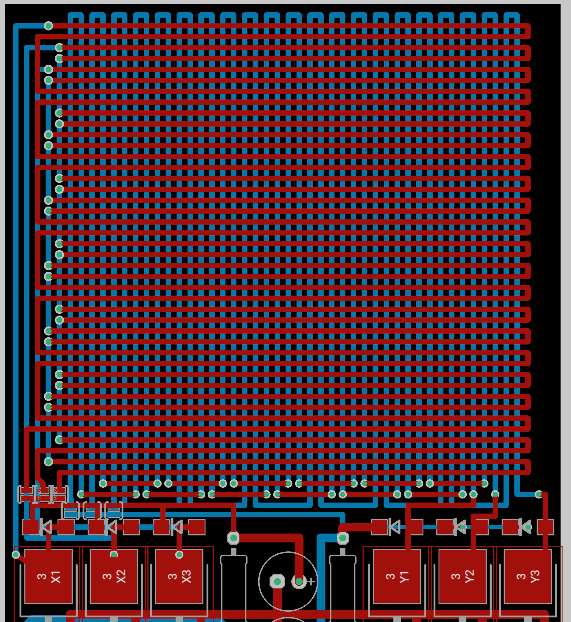
\includegraphics[width=0.8\linewidth]{2d_all_traces.png}
	\caption[\gls{pcb} design 2D actuator]{\gls{pcb} design with linear coils Source: hackaday.io ref: URL06}
	\label{fig:2d_all_traces}
\end{figure}

We can see three different traces running on all the \gls{pcb} and alternating. There is three of these traces on the TOP layer of the \gls{pcb} and three on the BOTTOM layer. The magnet is moved by passing current through each coil one by one. The direction of the magnet is determined by the order of activation of the coils. So by activating the coils one then two then three, the magnet will move in one direction. By activating the coils three then two then one, the magnet will move in the opposite direction.

\begin{figure}[H]
	\centering
	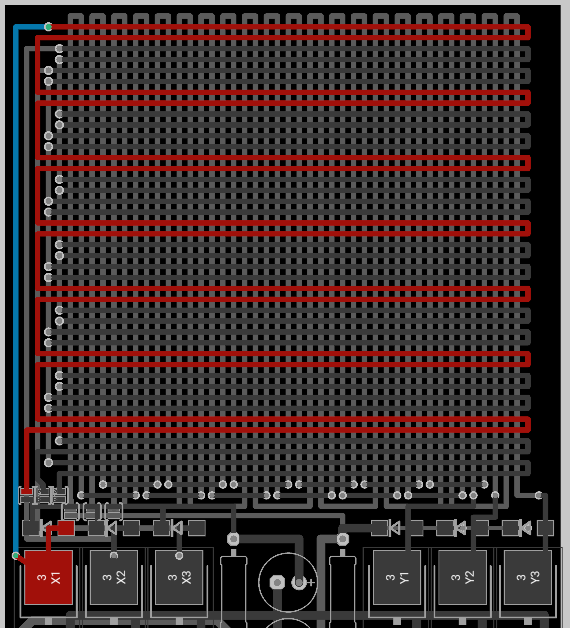
\includegraphics[width=0.6\linewidth]{2d_horizontal_trace.png}
	\caption[\gls{pcb} design horizontal traces]{\gls{pcb} design with horizontal coils}
	\label{fig:2d_horizontal_traces}
\end{figure}

\begin{figure}[H]
	\centering
	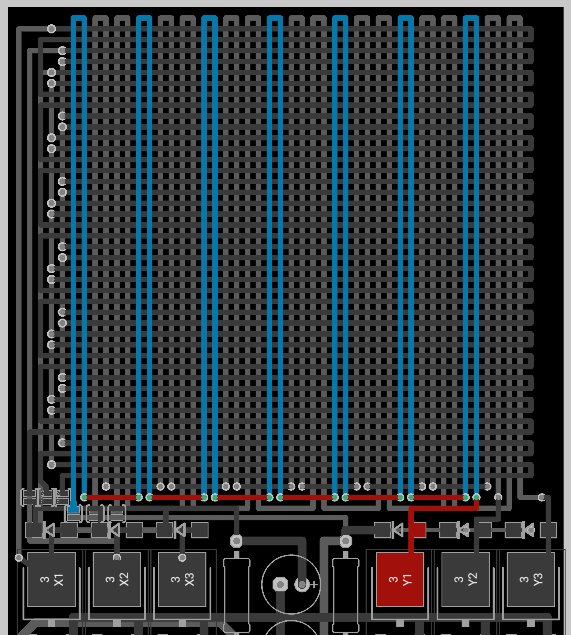
\includegraphics[width=0.6\linewidth]{2d_vertical_trace.png}
	\caption[\gls{pcb} design vertical traces]{\gls{pcb} design with vertical coils}
	\label{fig:2d_vertical_traces}
\end{figure}

\section{PCB coils}

Some projects use \gls{pcb} traces to draw arbitrary shaped coils like spirals or squares to generate a magnetic field. They can increase the torque by increasing the number of turns or current capacity (Bigger traces means less resistance, which means more current thus more magnetic field). They can also enhance the magnetic field by stacking multiple coils on the different \gls{pcb} layers.

Unlike the pcb stator motors where the magnets are on a free rotating shaft, the coils here have to generate enough force to attract the magnet while countering the friction between the magnet and the \gls{pcb}.

Carl Bugeja\footcite{noauthor_carl_nodate} has made a project where he uses a spiral coil to move a magnet in a linear path, he actually the design with FR4\footcite{noauthor_fr-4_2024} basic \gls{pcb} but also with flexible \gls{pcb}. He made a small video\footcite{carl_bugeja_actuating_2018} of the magnet moving on the \gls{pcb}. He mostly uses a Ball magnet to help reduce the friction between the magnet and the \gls{pcb}.

\begin{figure}[H]
	\centering
	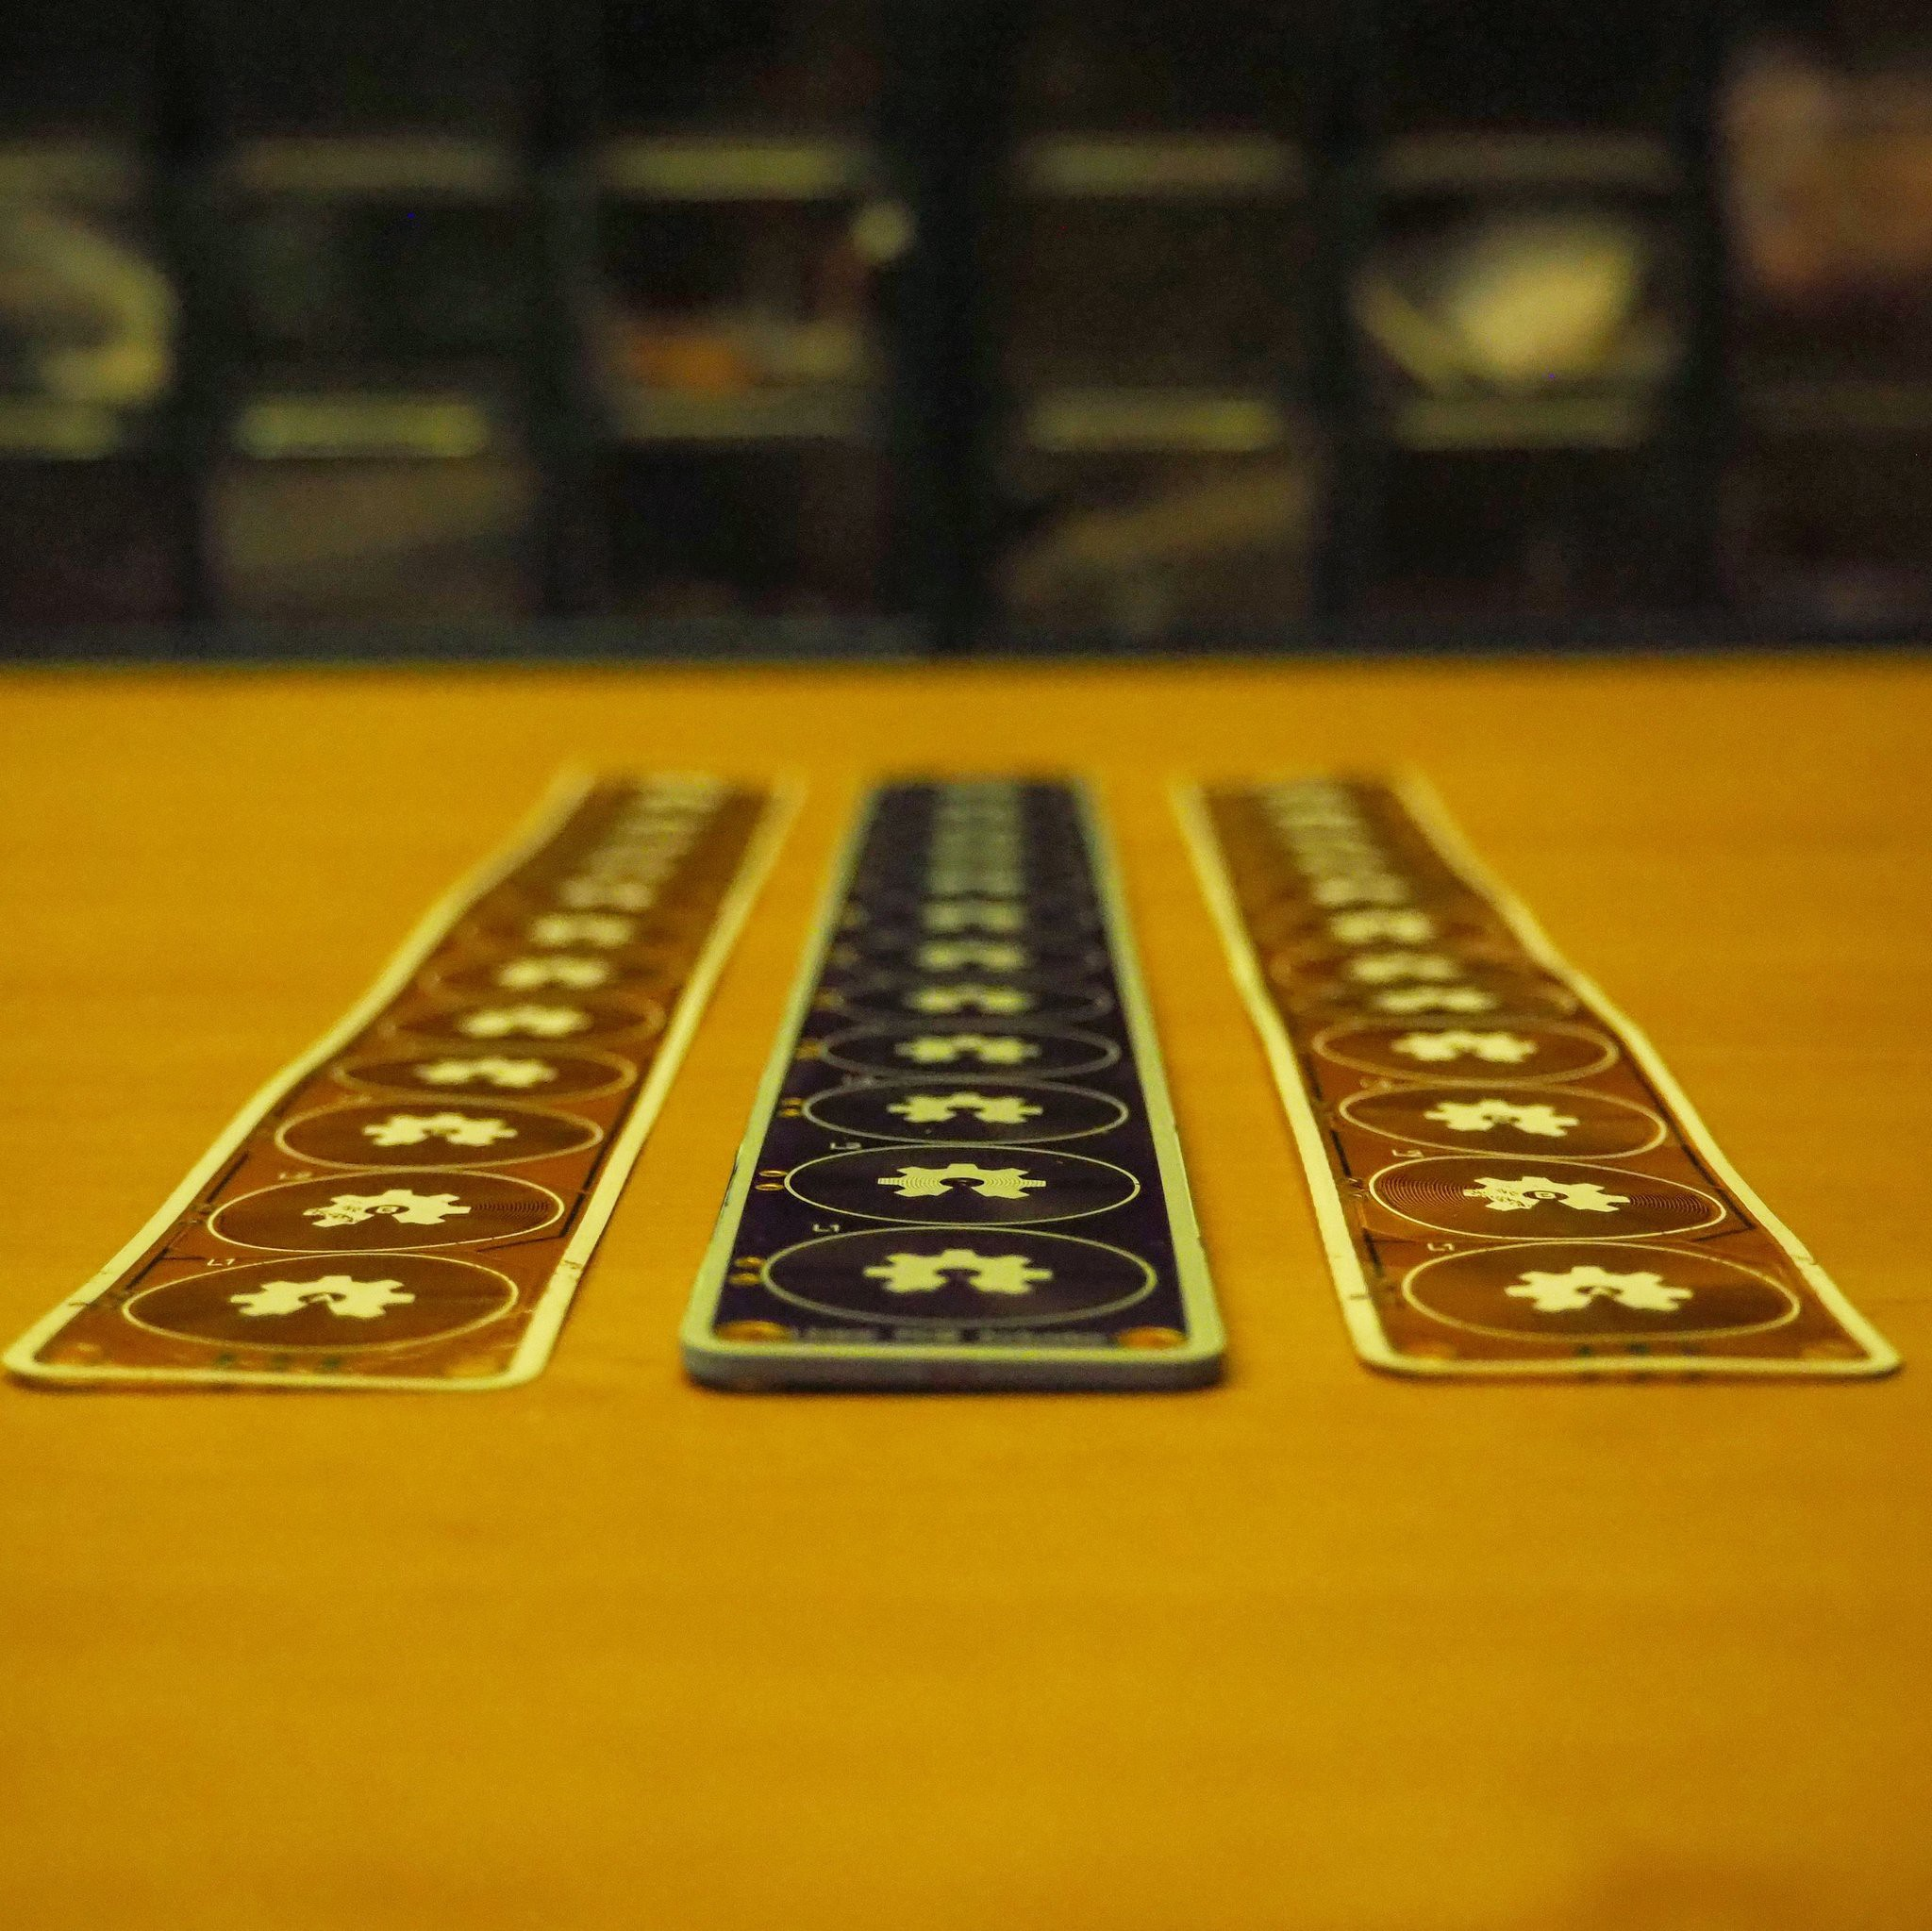
\includegraphics[width=0.6\linewidth]{pcb_coils.jpg}
	\caption[\gls{pcb} coils design from Carl Bugeja]{\gls{pcb} design of spiraling coils that form a linear path for a magnet Source: hackaday.io ref: URL07}
	\label{fig:pcb_coils_spiral}
\end{figure}




%\begin{figure}[H]
%	\centering
%	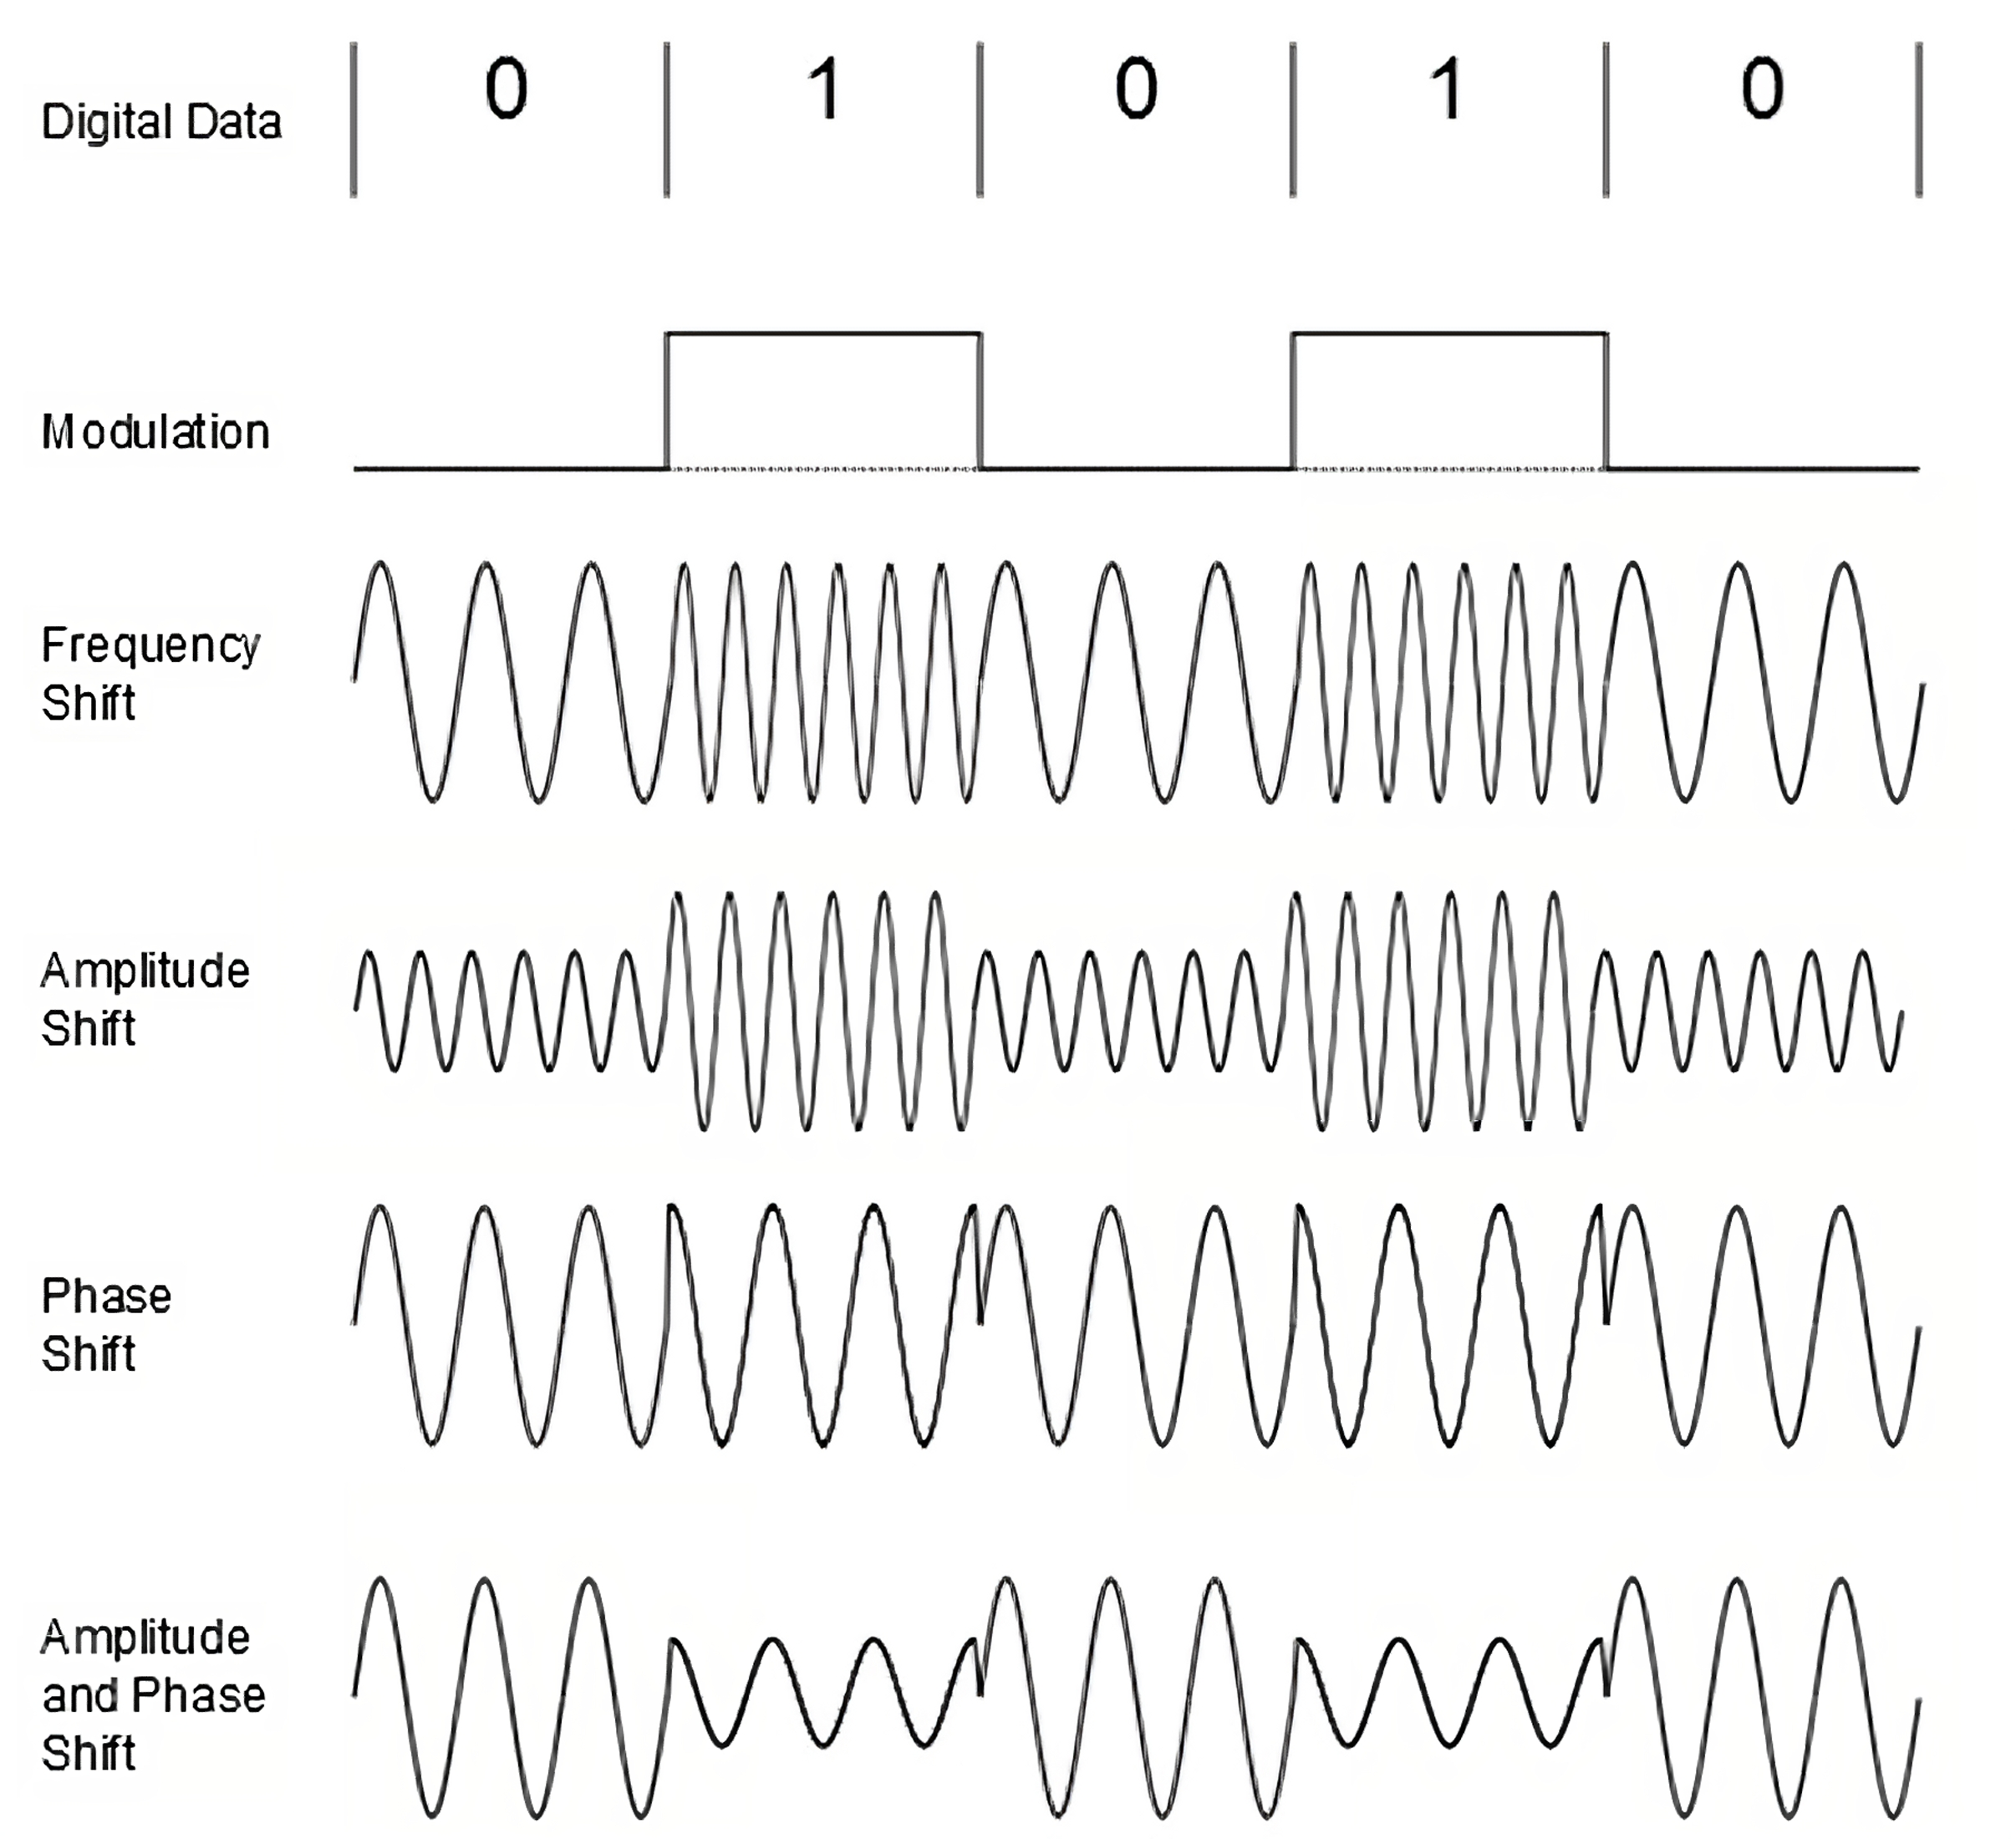
\includegraphics[width=0.8\linewidth]{modulations.png}
%	\caption[Modulations]{Example of modulations Source: https://content.cdntwrk.com/ ref: URL06}
%	\label{fig:modulations}
%\end{figure}


